\section{Phoenix internals}

\frame{\tableofcontents[currentsection]}

\begin{frame}
    \frametitle{Phoenix layers}
    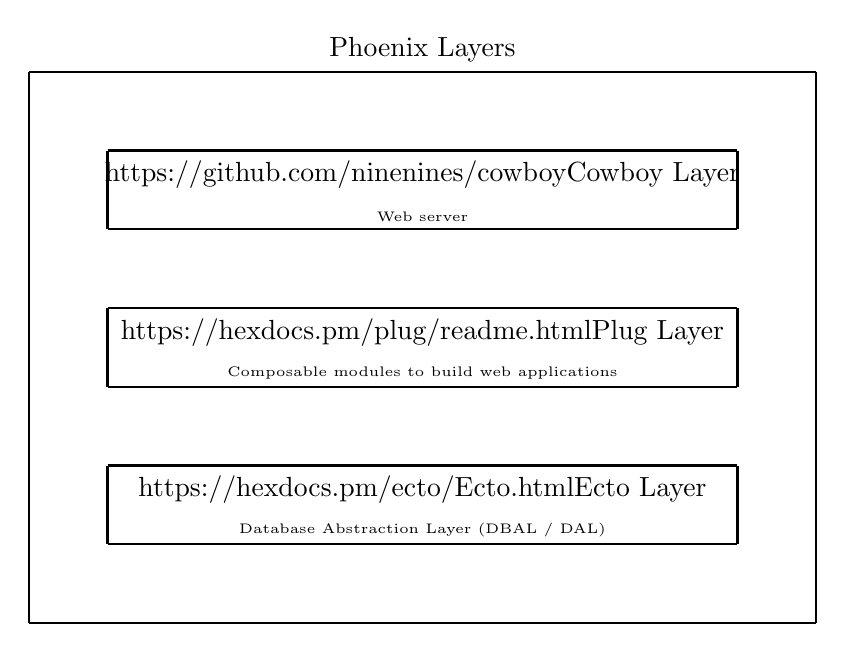
\begin{tikzpicture}
        % TODO: refactor https://www.overleaf.com/learn/latex/LaTeX_Graphics_using_TikZ:_A_Tutorial_for_Beginners_(Part_1)%E2%80%94Basic_Drawing
        % ############### OUTER BOX START ##################
        % Upper horizontal line with phoenix text
        \draw[thick] (0,2) -- node[above] {Phoenix Layers} (10,2);
        % Lower horizontal line
        \draw[thick] (0,-5) -- (10,-5);

        % Left vertical line
        \draw[thick] (0,2) -- (0,-5);
        % Right vertical line
        \draw[thick] (10,2) -- (10,-5);

        % ############### OUTER BOX END ####################

        % ############### LAYER COWBOY START ###############
        % Upper horizontal line with cowboy layer
        \draw[thick] (1,1) -- node[below] {\href{https://github.com/ninenines/cowboy}{Cowboy Layer}} (9,1);
        % Lower horizontal line
        \tiny
        \draw[thick] (1,0) -- node[above] {Web server} (9,0);
        \normalsize
        % Left vertical line
        \draw[thick] (1,1) -- (1,0);
        % Right vertical line
        \draw[thick] (9,1) -- (9,0);
        % ############### LAYER COWBOY END #################

        % ############### LAYER PLUG START #################
        % Upper horizontal line with plug layer
        \draw[thick] (1,-1) -- node[below] {\href{https://hexdocs.pm/plug/readme.html}{Plug Layer}} (9,-1);
        % Lower horizontal line
        \tiny
        \draw[thick] (1,-2) -- node[above] {Composable modules to build web applications} (9,-2);
        \normalsize
        % Left vertical line
        \draw[thick] (1,-1) -- (1,-2);
        % Right vertical line
        \draw[thick] (9,-1) -- (9,-2);
        % ############### LAYER PLUG END ###################

        % ############### LAYER ECTO START #################
        % Upper horizontal line with Ecto layer
        \draw[thick] (1,-3) -- node[below] {\href{https://hexdocs.pm/ecto/Ecto.html}{Ecto Layer}} (9,-3);
        % Lower horizontal line
        \tiny
        \draw[thick] (1,-4) -- node[above] {Database Abstraction Layer (DBAL / DAL)} (9,-4);
        \normalsize
        % Left vertical line
        \draw[thick] (1,-3) -- (1,-4);
        % Right vertical line
        \draw[thick] (9,-3) -- (9,-4);
        % ############### LAYER ECTO END ###################
    \end{tikzpicture}
\end{frame}


\begin{frame}
    \frametitle{\href{https://hexdocs.pm/phoenix/request_lifecycle.html}{Request lifecycle}}
    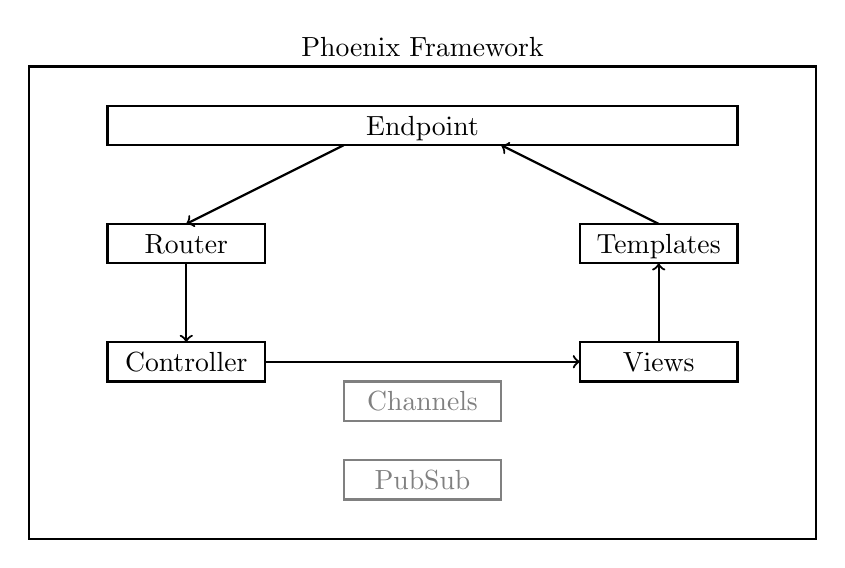
\begin{tikzpicture}

        \draw[thick] (0,2) -- node[above] {Phoenix Framework}
        (10,2) -- (10,-4) -- (0,-4) -- cycle;

        \draw[thick] (1,1.5) -- node[below] {Endpoint}
        (9,1.5) -- (9,1) -- (1,1) -- cycle;

        \draw[thick] (1,0) -- node[below] {Router}
        (3,0) -- (3,-0.5) -- (1,-0.5) -- cycle;

        \draw[thick] (1,-1.5) -- node[below] {Controller}
        (3,-1.5) -- (3,-2) -- (1,-2) -- cycle;

        \draw[thick] (7,-1.5) -- node[below] {Views}
        (9,-1.5) -- (9,-2) -- (7,-2) -- cycle;

        \draw[thick] (7,-0) -- node[below] {Templates}
        (9,-0) -- (9,-0.5) -- (7,-0.5) -- cycle;

        \draw[thick, gray] (4,-2) -- node[below] {Channels}
        (6,-2) -- (6,-2.5) -- (4,-2.5) -- cycle;

        \draw[thick, gray] (4,-3) -- node[below] {PubSub}
        (6,-3) -- (6,-3.5) -- (4,-3.5) -- cycle;

        % #######################################

        \draw[->, thick] (4,1) -- (2,0);
        \draw[->, thick] (2,-0.5) -- (2,-1.5);
        \draw[->, thick] (3,-1.75) -- (7,-1.75);
        \draw[->, thick] (8,-1.5) -- (8,-0.5);
        \draw[->, thick] (8,0) -- (6,1);

    \end{tikzpicture}
\end{frame}

\begin{frame}
    \frametitle{Websocket communication (soft-realtime)}
    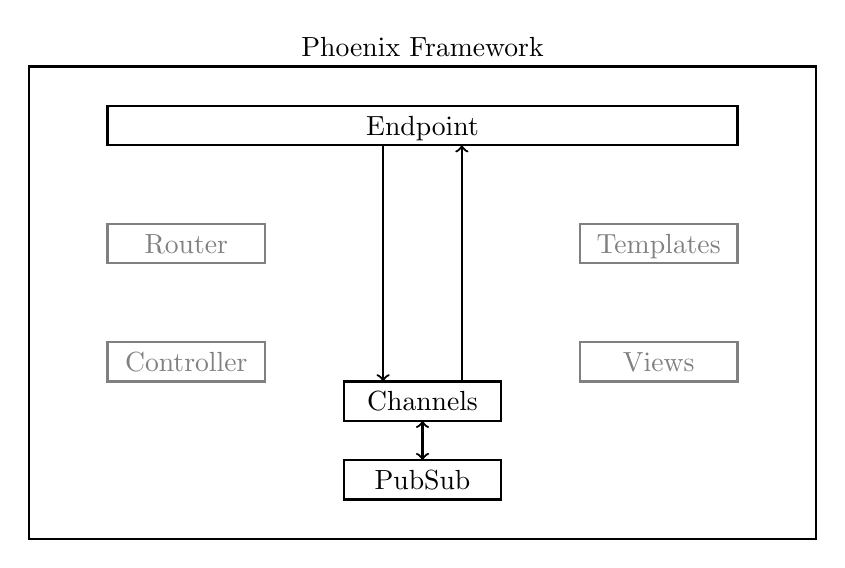
\begin{tikzpicture}

        \draw[thick] (0,2) -- node[above] {Phoenix Framework}
        (10,2) -- (10,-4) -- (0,-4) -- cycle;

        \draw[thick] (1,1.5) -- node[below] {Endpoint}
        (9,1.5) -- (9,1) -- (1,1) -- cycle;

        \draw[thick, gray] (1,0) -- node[below] {Router}
        (3,0) -- (3,-0.5) -- (1,-0.5) -- cycle;

        \draw[thick, gray] (1,-1.5) -- node[below] {Controller}
        (3,-1.5) -- (3,-2) -- (1,-2) -- cycle;

        \draw[thick, gray] (7,-1.5) -- node[below] {Views}
        (9,-1.5) -- (9,-2) -- (7,-2) -- cycle;

        \draw[thick, gray] (7,-0) -- node[below] {Templates}
        (9,-0) -- (9,-0.5) -- (7,-0.5) -- cycle;

        \draw[thick] (4,-2) -- node[below] {Channels}
        (6,-2) -- (6,-2.5) -- (4,-2.5) -- cycle;

        \draw[thick] (4,-3) -- node[below] {PubSub}
        (6,-3) -- (6,-3.5) -- (4,-3.5) -- cycle;

        % #######################################

        \draw[->, thick] (4.5,1) -- (4.5,-2);
        \draw[->, thick] (5.5,-2) -- (5.5,1);

        \draw[->, thick] (5,-2.5) -- (5,-3);
        \draw[->, thick] (5,-3) -- (5,-2.5);

    \end{tikzpicture}
\end{frame}

\begin{frame}
    \frametitle{Libraries explanation 1/3}
    \structure{Endpoint}
    \begin{itemize}
        \item start and end of the request lifecycle
        \item all aspects of requests up until the router takes over
        \item core set of plugs to apply to all requests
    \end{itemize}

    \vfill

    \structure{Router}
    \begin{itemize}
        \item parses and dispatches requests to the correct controller/action
        \item helpers to generate route paths or urls to resources
        \item pipelines - applies groups of plugs to a set of routes
    \end{itemize}

    \vfill

    \structure{Controller}
    \begin{itemize}
        \item provide functions, called actions, to handle requests
        \item action: prepare data and pass it into views
        \item action: invoke rendering via views 
        \item action: perform redirects 
    \end{itemize}
\end{frame}

\begin{frame}
    \frametitle{Libraries explanation 2/3}
    \structure{Views - presentation layer}
    \begin{itemize}
        \item render templates
        \item define template helper functions to decorate data
    \end{itemize}

    \vfill

    \structure{Templates}
    \begin{itemize}
        \item files containing the contents that will be served in a response
        \item basic response structure, allow dynamic data to be inserted
        \item precompiled and fast
    \end{itemize}
\end{frame}

\begin{frame}
    \frametitle{Libraries explanation 3/3}

    \structure{Channels}
    \begin{itemize}
        \item manage sockets for easy realtime communication
        \item analogous to controllers, but allow bi-directional communication with persistent connections
    \end{itemize}

    \vfill

    \structure{PubSub}
    \begin{itemize}
        \item underlies the channel layer and allows clients to subscribe to topics
    \end{itemize}
\end{frame}